
\section{Données}
%%%%%%%%%%%%%%%%%%%%%%%%%%%%%%%%%%%%%%%%%%%%%%%%%%%%%%%%%%%%%%%%%%%%%%%
\subsection{Présentation}

Nous disposons de deux séries de données contenues dans le package \lstinline!gumbel! correspondant à la vitesse maximale du vent par jour, sur la période août 2005 - avril 2007,
relevée à deux stations différentes en région Rhône-Alpes : l'une à Saint Martin en haut (département du Rhône) et et une autre à Echirolles (département de l'Isère).

~\\~
Notons :
\begin{itemize}
\item $(X_t)_t$ la série relative à la force maximale du vent (en m/s) par jour relevée par la station à Saint Martin en Haut 
\item $(Y_t)_t$ la série relative à la force maximale du vent (en m/s) par jour relevée par la station à Echirolles.
\end{itemize}

~\\~
Puisque les jeux de données appelés dans $R$ \lstinline!windEchirolles! et \lstinline!windStMartin! possèdent 
un nombre d’enregistrements différents en 2007, nous sélectionnons le plus petit sous-ensemble. Les données manquantes sont aussi retirées de la série.

Nous avons ainsi deux vecteurs de données contenant chacun $T=633$ données (correspondant à 633 jours).


\subsection{Formalisation}

Nous allons donc nous intéresser à la relation existant entre ces deux variables aléatoires réelles au moyen de modélisations par copules.
En effet,  les fonctions copules permettent de déterminer la nature de dépendance des séries qu’elle soit linéaire ou pas, monotone ou pas.

D'une manière explicite, les copules sont des fonctions de répartition particulières,
qui lient les fonctions de répartition multivariéees de lois de probabilitée dans $\mathbb{R}^d$, où $d \geq 2$ (ici $d$ sera égal à 2 car nous aurons un modèle bivarié) aux fonctions de répartition marginales de leurs coordonnées. 
La caractéristique des copules permet de séparer les distributions marginales de la structure de dépendance.

Plus précisément, $X$ et $Y$  sont définies sur un espace de probabilité $(\Omega,\mathcal{A},\mathbb{P})$, de fonction de répartition conjointe $H$ et de marginales $F$ et $G$.

D'après Sklar (1959), il existe une fonction de répartition bivariée $C$ dont les marges sont uniformes sur $[0,1]$, telle que :
$$
H(x,y) = C(F(x),G(y))
$$

De plus, si $F$ et $G$ sont continues, la copule $C$ est alors unique et on a :

$$
\forall (u,v) \in [0,1]^2 ~~ C(u,v) = H(F^{-1}(u),G^{-1}(v))
$$

En fait, il s'agit de la loi du couple $(U,V) = (F(X),G(Y))$.

Nous allons donc chercher la copule qui s’adapte le mieux à nos données.




\subsection{Observation graphique}



\subsubsection{Scatter plot}




\subsubsection{Rank-rank plot}

\subsection{Mesurer la dépendance}

\subsubsection{Dépendance ou corrélation ?}

Il est important de rappeler que les notions de dépendance et de corrélation sont différentes.
En effet, si $X$ et $Y$ sont indépendantes, cela implique que $X$ et $Y$ sont non corrélées. Mais attention, la réciproque est fausse, sauf dans
le cas où les variables sont gaussiennes car la dépendance est alors entièrement caractérisées par le coefficient de corrélation.

Un contre-exemple permettant d'illustrer cette remarque est le suivant :

Soit $X \sim \mathcal{N}(0,1)$ et $Y = X^2$, alors $\operatorname{Cov}(X,Y) = E[X^3] = 0$.

Le coefficient de corrélation doit donc être utilisée avec précaution car il n’est pertinent qu’en présence de distributions elliptiques (distribution multivariée
Normale ou de Student) ou de dépendance linéaire.


\subsubsection{Corrélation de Pearson}

Le coefficient de corrélation linéaire de Pearson est défini, pour nos deux variables aléatoires $X$ et $Y$ de variances finies, par :

$$
r(X,Y) = \frac{\operatorname{Cov}(X,Y)}{\sqrt{ \operatorname{Var}(X) \operatorname{Var}(Y)}}
$$

où $\operatorname{Cov}(X,Y) = E[XY] - E[X] E[Y]$ est la covariance entre $X$ et $Y$ et $\operatorname{Var}(X)$, $\operatorname{Var}(Y)$ correspondent aux variances respectives
de $X$ et $Y$.

Le coefficient de corrélation de Pearson est la mesure la plus connue. Mais il constitute une mesure très imparfaite de la dépendance. Il ne
peut se mettre sous une forme ne faisant intervenir que la copule, les marginales restent présentent dans l’expression : ce coefficient n’est donc
pas une mesure de dépendance.

De plus, il n’intègre que la composante linéaire de la dépendance, au sens où $r(X,Y) \pm 1$ si et seulement si $Y= a \times x + b$.

Enfin, on peut montrer (en utilisant l'inégalité de Tchen) que, pour les marginales fixées, toutes les valeurs
comprises entre -1 et +1 ne sont pas atteignables.

Ainsi, on retiendra que ce coefficient mesure mal une association non-linéaire, qu'il est trop sensible aux valeurs extrêmes et qu'il ne mesure pas vraiment la distance à l'indépendance.


\subsubsection{Rho de Spearman}



\subsubsection{Tau de Kendall}



\section{Méthode non paramétrique d'estimation : la copule empirique}
%%%%%%%%%%%%%%%%%%%%%%%%%%%%%%%%%%%%%%%%%%%%%%%%%%%%%%%%%%%%%%%%%%%%%%%
\subsection{Choix d'une copule théorique}




\section{Méthode paramétriques d'estimation}
%%%%%%%%%%%%%%%%%%%%%%%%%%%%%%%%%%%%%%%%%%%%%%%%%%%%%%%%%%%%%%%%%%%%%%%

Dans cette section, nous allons présenter et utiliser deux méthodes paramétriques d'estimation
des copules :

\begin{itemize}
\item la méthode du maximum de vraisemblance
\item la méthode IFM (Inference Function for Margins).
\end{itemize}

\subsection{Méthode du maximum de vraisemblance}

\subsection{Méthode IFM (Inference Function for Margins)}


\section{Méthode semi-paramétrique d'estimation (CML)}
%%%%%%%%%%%%%%%%%%%%%%%%%%%%%%%%%%%%%%%%%%%%%%%%%%%%%%%%%%%%%%%%%%%%%%%

Dans cette section, nous allons utiliser la méthode CML (méthode semi-paramétrique) afin d'estimer le paramètre des différentes copules retenues pour modéliser la dépendance entre les données sur Saint-Martin et celles sur Echirolles.
En effet, à l'aide de cette méthode, on peut obtenir une estimation du paramètre de la copule sans se soucier des marginales. Pour cela, il suffit d'utiliser la fonction \textit{fitcopula} de R en passant comme arguments les rangs sur nos deux groupes de données translatés sur $[0;1]$ et un point de départ de l'algorithme. Ce point de départ sera l'estimation du paramètre de la copule obtenue par la méthode des moments. Avec l'estimation du paramètre obtenue en sortie de notre algorithme, on peut alors créer notre copule estimée.

\subsection{Copule de Clayton}

Dans le cas de la copule de Clayton, on obtient, en sortie de l'algorithme, $\widehat{\theta}_{CML}=0,6890$ comme estimation du paramètre de la copule. L'écart type pour cet estimateur vaut $sd = 0,066$. La valeur obtenue pour l'estimation du paramètre est donc significative. Le maximum de vraisemblance est de $68,87$. 
On peut ainsi tracer les Khi-plot et K-plot de cette copule de Clayton estimée et comparer les graphes avec ceux obtenus pour la copule empirique.

\noindent%
\begin{figure}[H]
    \begin{center}
      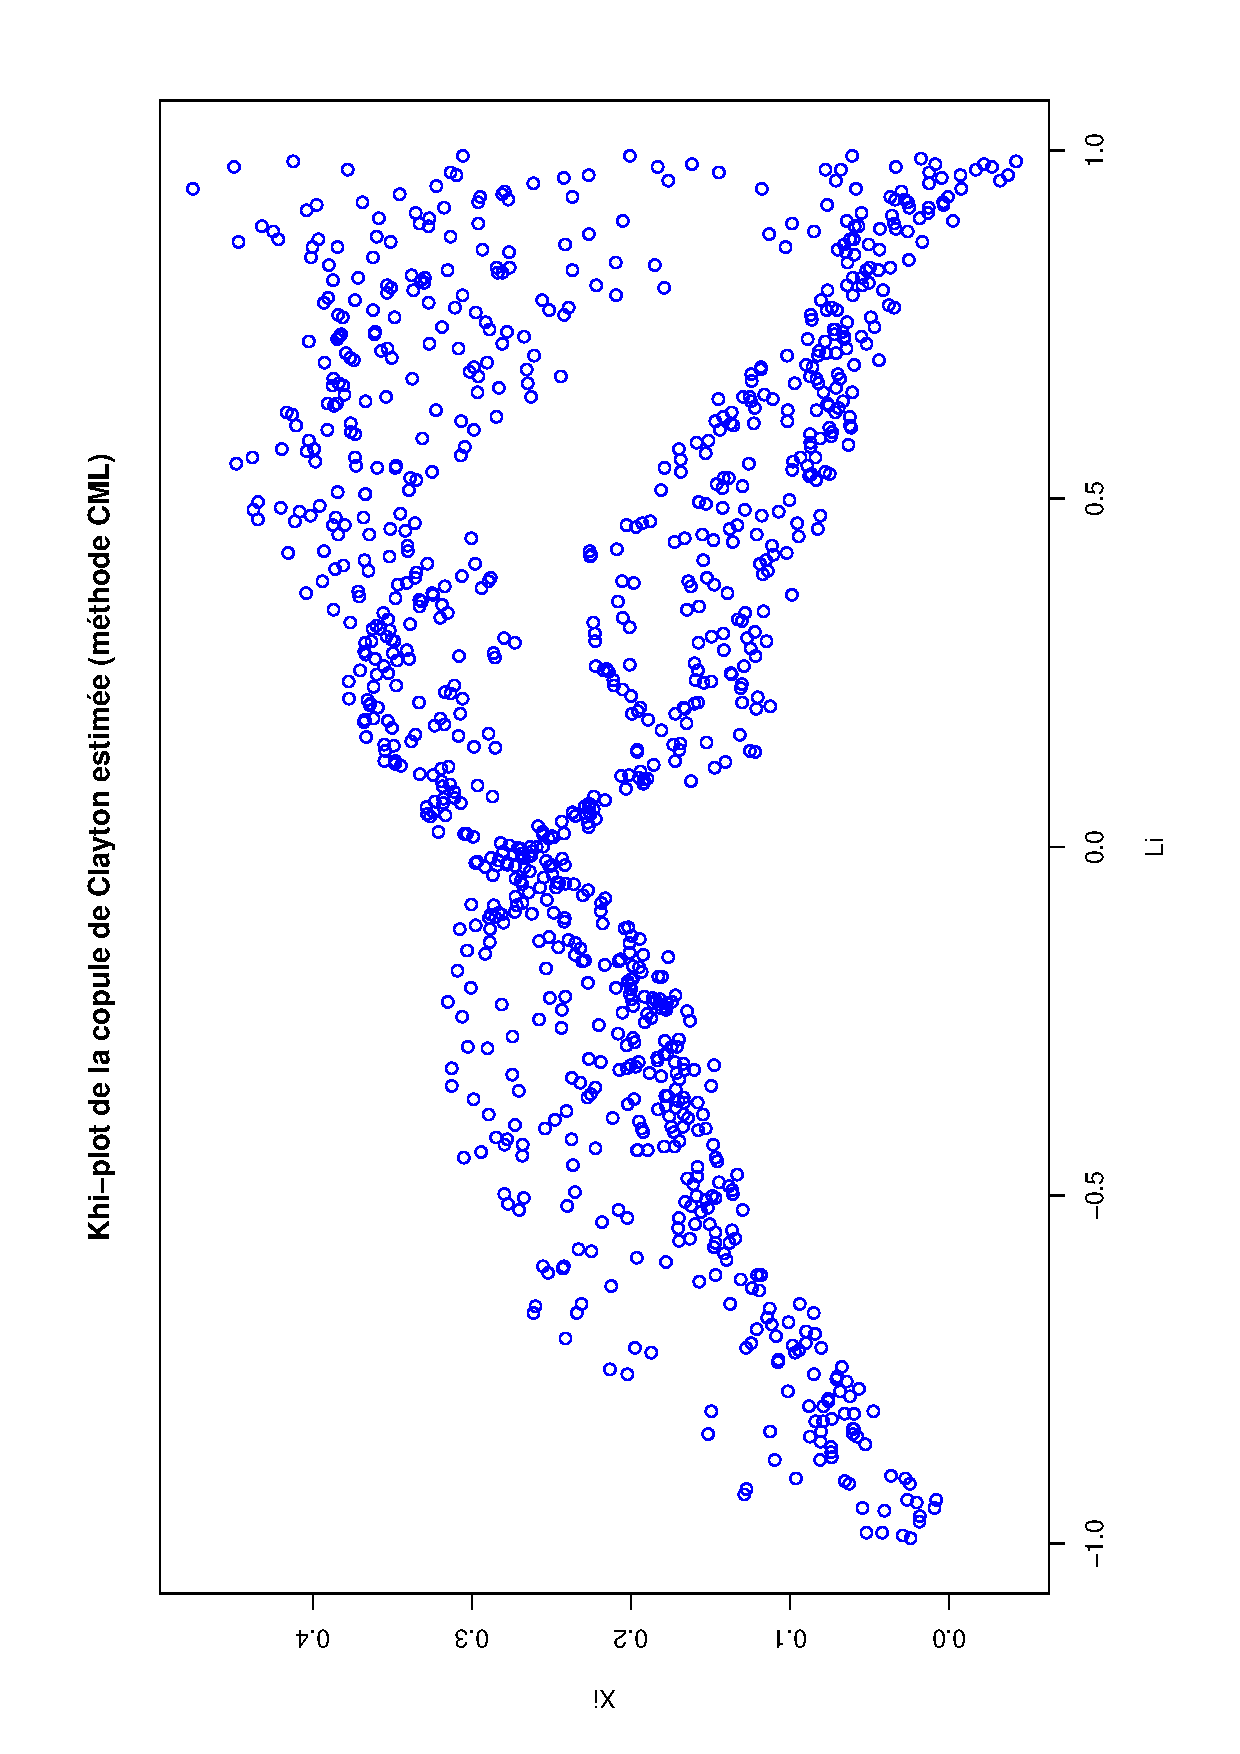
\includegraphics[width=17 cm, angle=0]{./pictures/claytoncmlkhiplot.png}
      \centering\caption{\label{2}Khi-plot de la copule de Clayton estimée (méthode CML)}
    \end{center}
\end{figure}

En comparant ce graphe du Khi-plot avec celui obtenu pour la copule empirique, on peut apercevoir une ressemblance, notamment dûe au fait que les points se répartissent du même côté de l'axe des ordonées (du côté positif) exprimant ainsi une dépendance positive. Cependant, du côté positif de l'axe des abscisses, le nuage de point semble se séparer en deux. Ceci n'est pas observée sur le khi-plot de la copule empirique. 

\noindent%
\begin{figure}[H]
    \begin{center}
      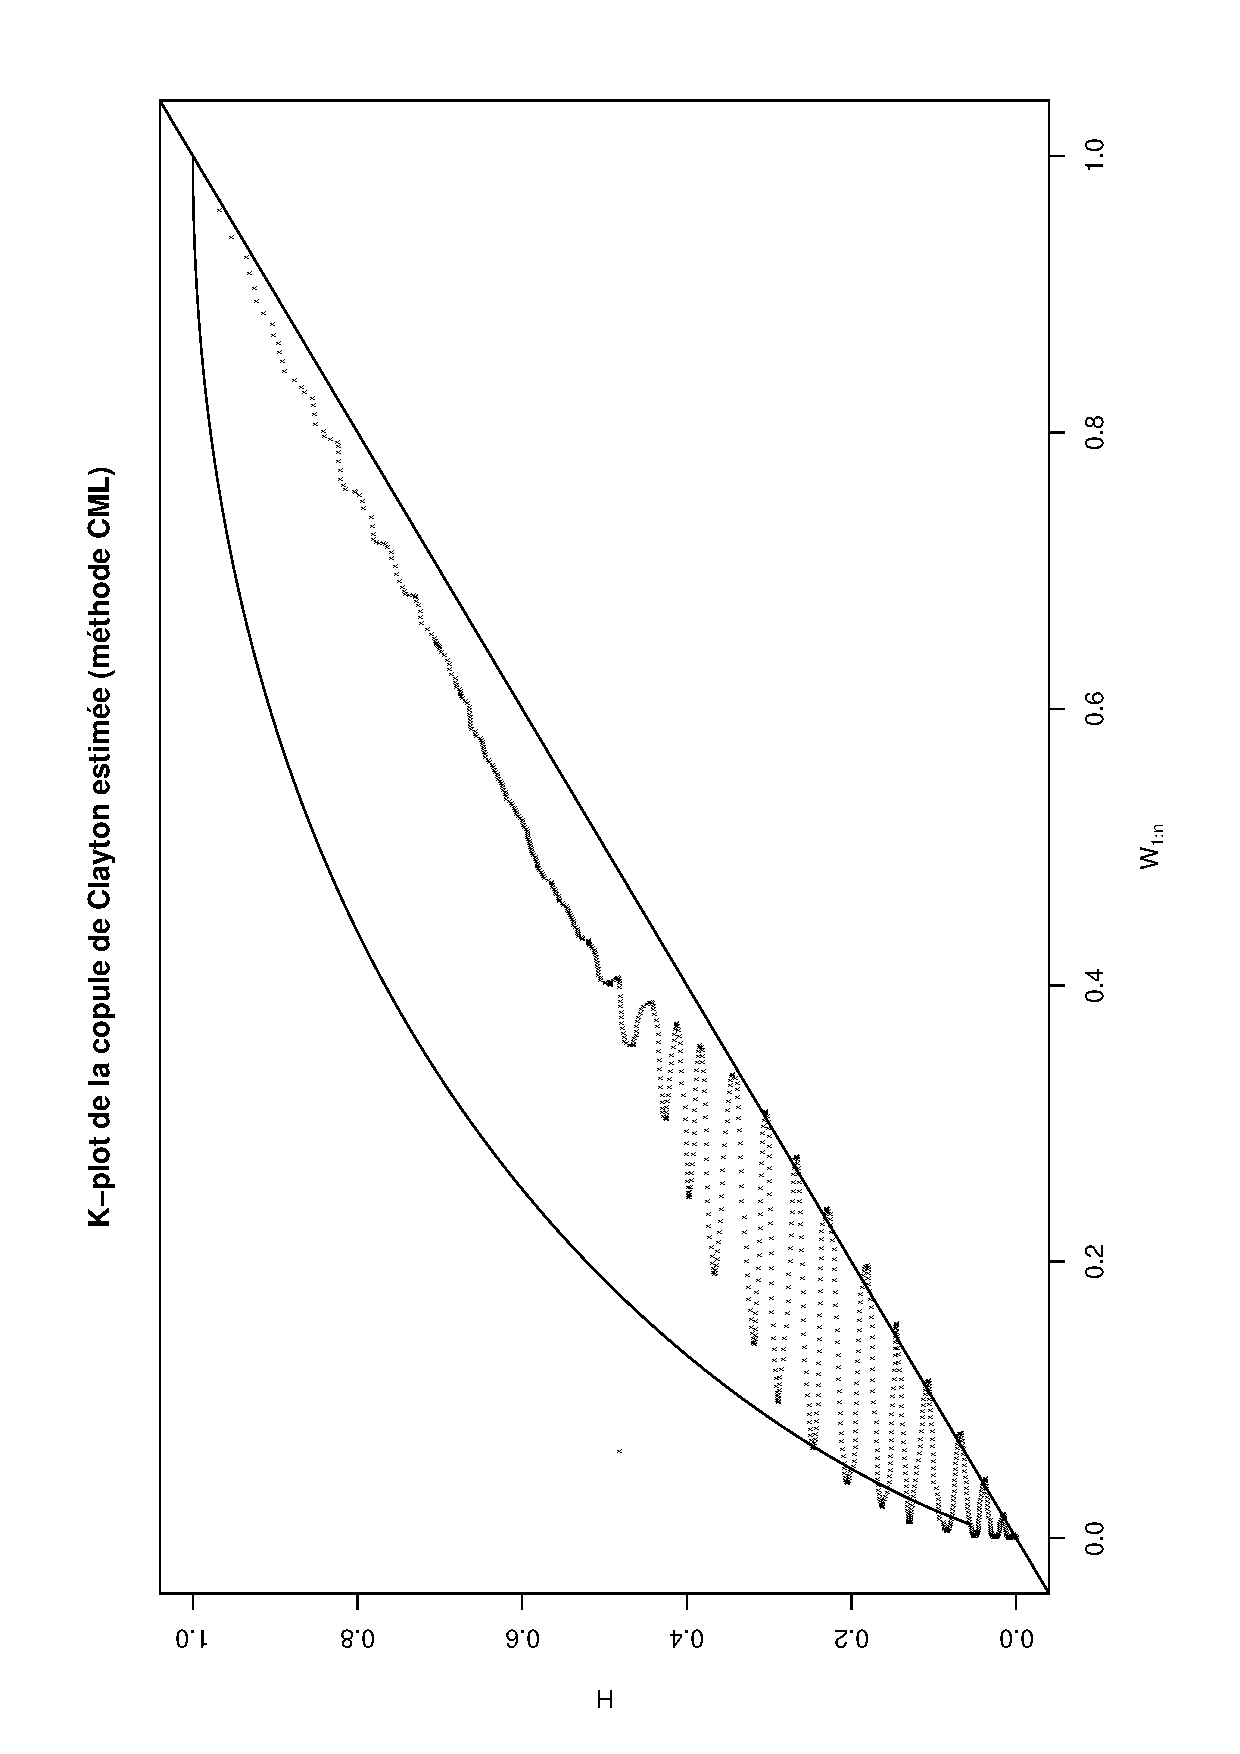
\includegraphics[width=17 cm, angle=0]{./pictures/claytoncmlkplot.png}
      \centering\caption{\label{2}K-plot de la copule de Clayton estimée (méthode CML)}
    \end{center}
\end{figure}

De la même manière, pour ce graphe du K-plot, on observe une similitude et plusieurs disparités par rapport à celui de la copule empirique. En effet, les points semblent se répartir dans le même espace pour les deux figures (globalement entre la courbe de dépendance positive parfaite et la droite d'indépendance $y=x$). Cela montre une nouvelle fois la dépendance positive entre nos deux séries de données. Cependant, concernant le graphe associé à la copule de Clayton estimée, les variations de la répartition des points sont plus grandes et plus nombreuses. Certains points dépassent en effet la courbe de dépendance positive parfaite et on compte également $14$ oscillations distinctes contre $12$ pour le K-plot de la copule empirique. De plus, pour les dernières espérances de statistique d'ordre, les points se rapprochent de la droite $y=x$ alors qu'ils sont proches de la courbe de dépendance positive parfaite pour le graphe concernant la copule empirique.

Ces graphes du Khi-plot et K-plot sont donc d'une certaine façon assez éloignés de ceux obtenus pour la copule empirique.

Pour prolonger nos résultats, on réalise également un algorithme de bootstrap paramétrique. Il s'agit de tester l'adéquation à notre modèle de copule. L'hypothèse nulle du test est donc la suivante:
$$
H_0 : C \in (C_{\theta})
$$
Avec $C_{\theta}$ la famille des copules de Clayton dans notre cas. 
En utilisant les mêmes notations que dans le cours, on rejette l'hypothèse nulle si $D_n > L$. 
Dans notre situation, on obtient, avec un seuil de $0,05$, $D_n = 0,1422 > 0,0463 = L$. De plus, la p-value pour cette statistique de Cramer-Von Mises vaut $0$. La copule empirique ne fait donc pas partie de la famille des copules de Clayton.

En conclusion de cette étude sur la copule de Clayton estimée, on peut considérer que la modélisation de la dépendance entre nos deux séries de données par une copule de Clayton n'est pas satisfaisante.

\subsection{Copule de Gumbel}

On procède de la même manière que pour la copule de Clayton. On obtient en sortie de l'algorithme une valeur de $\widehat{\theta}_{CML}=1,4644$ comme estimation du paramètre de la copule de Gumbel par la méthode CML. On a également la valeur de l'écart type $sd = 0,0548$. L'estimation obtenue est ainsi significative. Le maximum de vraisemblance vaut $92,59$.

On représente ainsi ci-dessous les graphes du Khi-plot et du K-plot de la copule de Gumbel estimée:

\noindent%
\begin{figure}[H]
    \begin{center}
      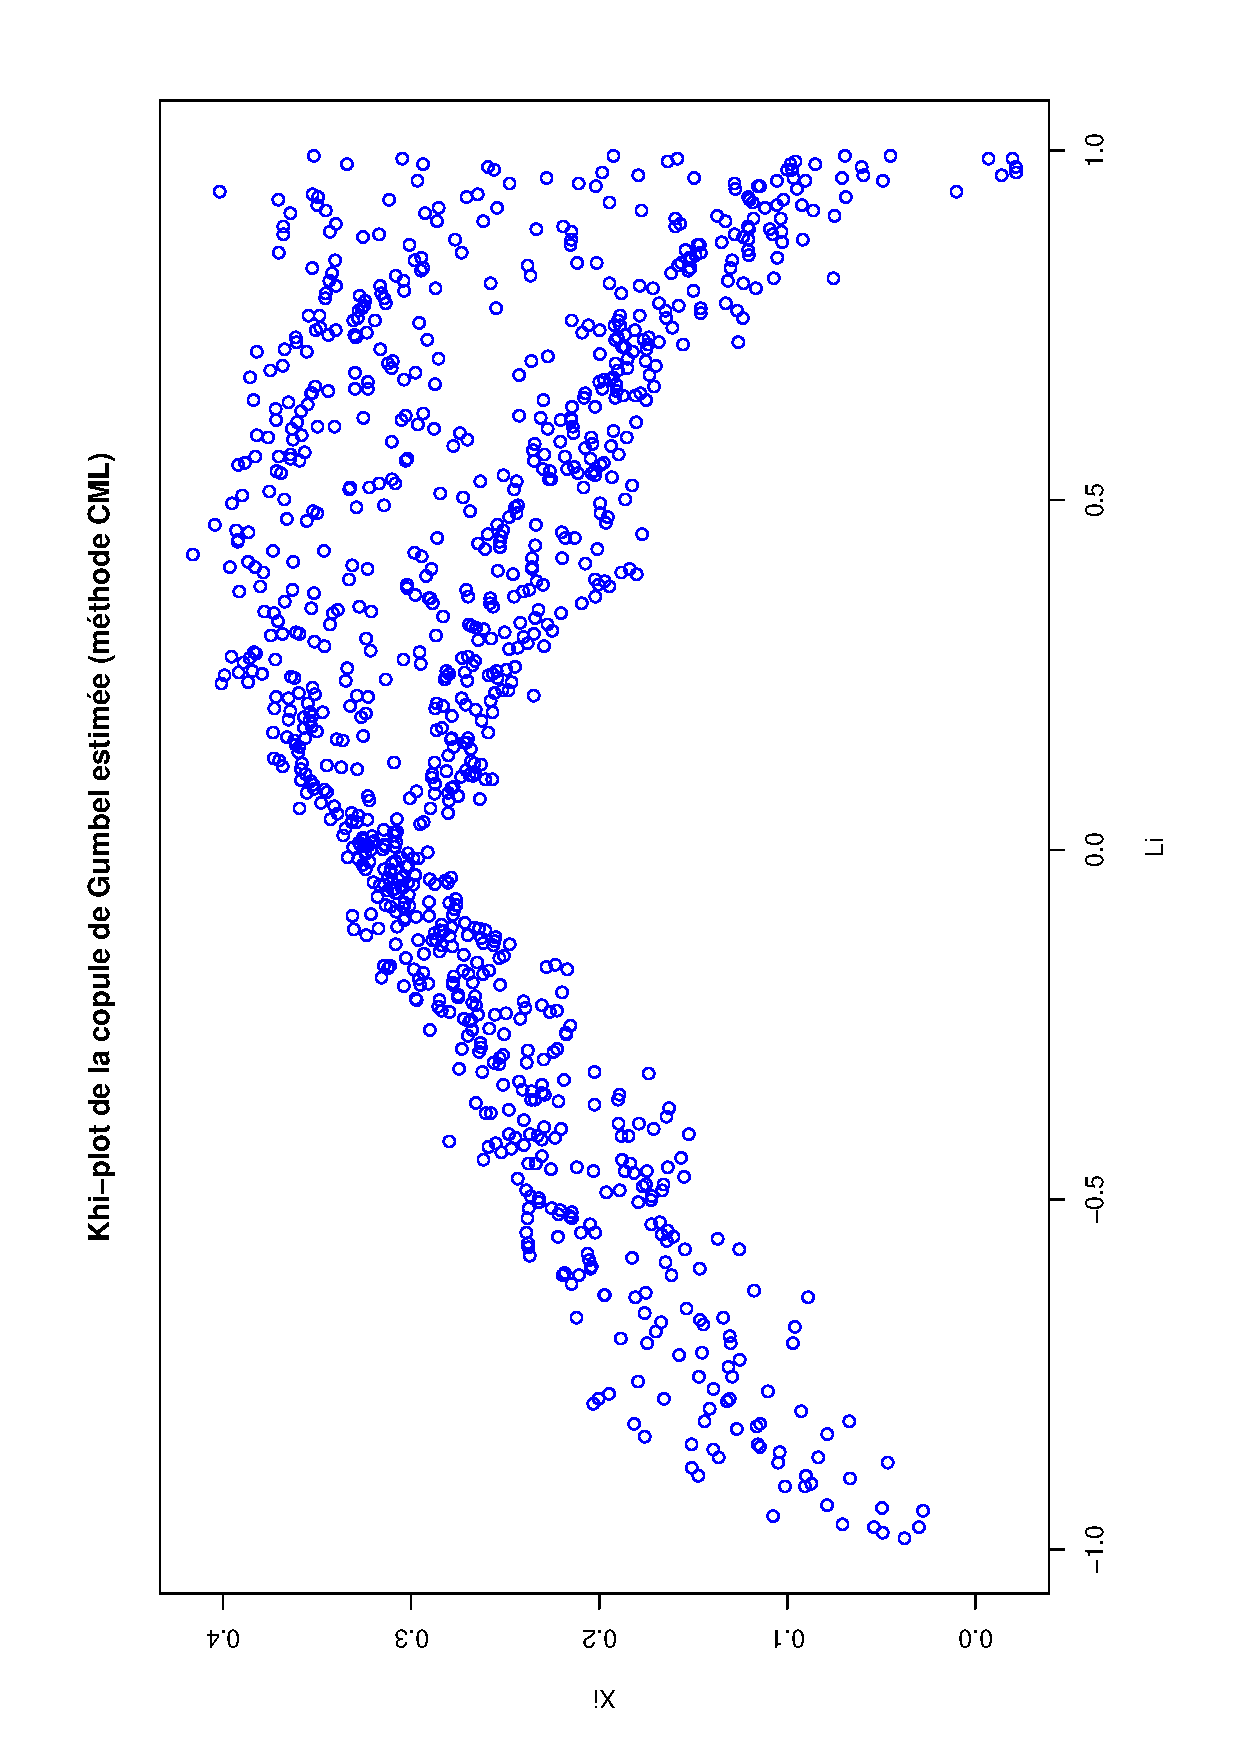
\includegraphics[width=17 cm, angle=0]{./pictures/gumbelcmlkhiplot.png}
      \centering\caption{\label{2}Khi-plot de la copule de Gumbel estimée (méthode CML)}
    \end{center}
\end{figure}

Le Khi-plot ci-dessus est très proche du Khi-plot obtenu avec la copule empirique. En effet, nous avons une répartition des points semblables. Le nuage de points est incurvée de la même manière du coté des valeurs positives des ordonnées et atteint une valeur maximale autour de $0,3$ comme pour le Khi-plot empirique. Certes, nous avons toujours une sorte de séparation en deux du nuage de points pour les valeurs positives en abscisse. Mais, cela est beaucoup moins prononcé que pour le Khi-plot de la copule de Clayton précédent.

\noindent%
\begin{figure}[H]
    \begin{center}
      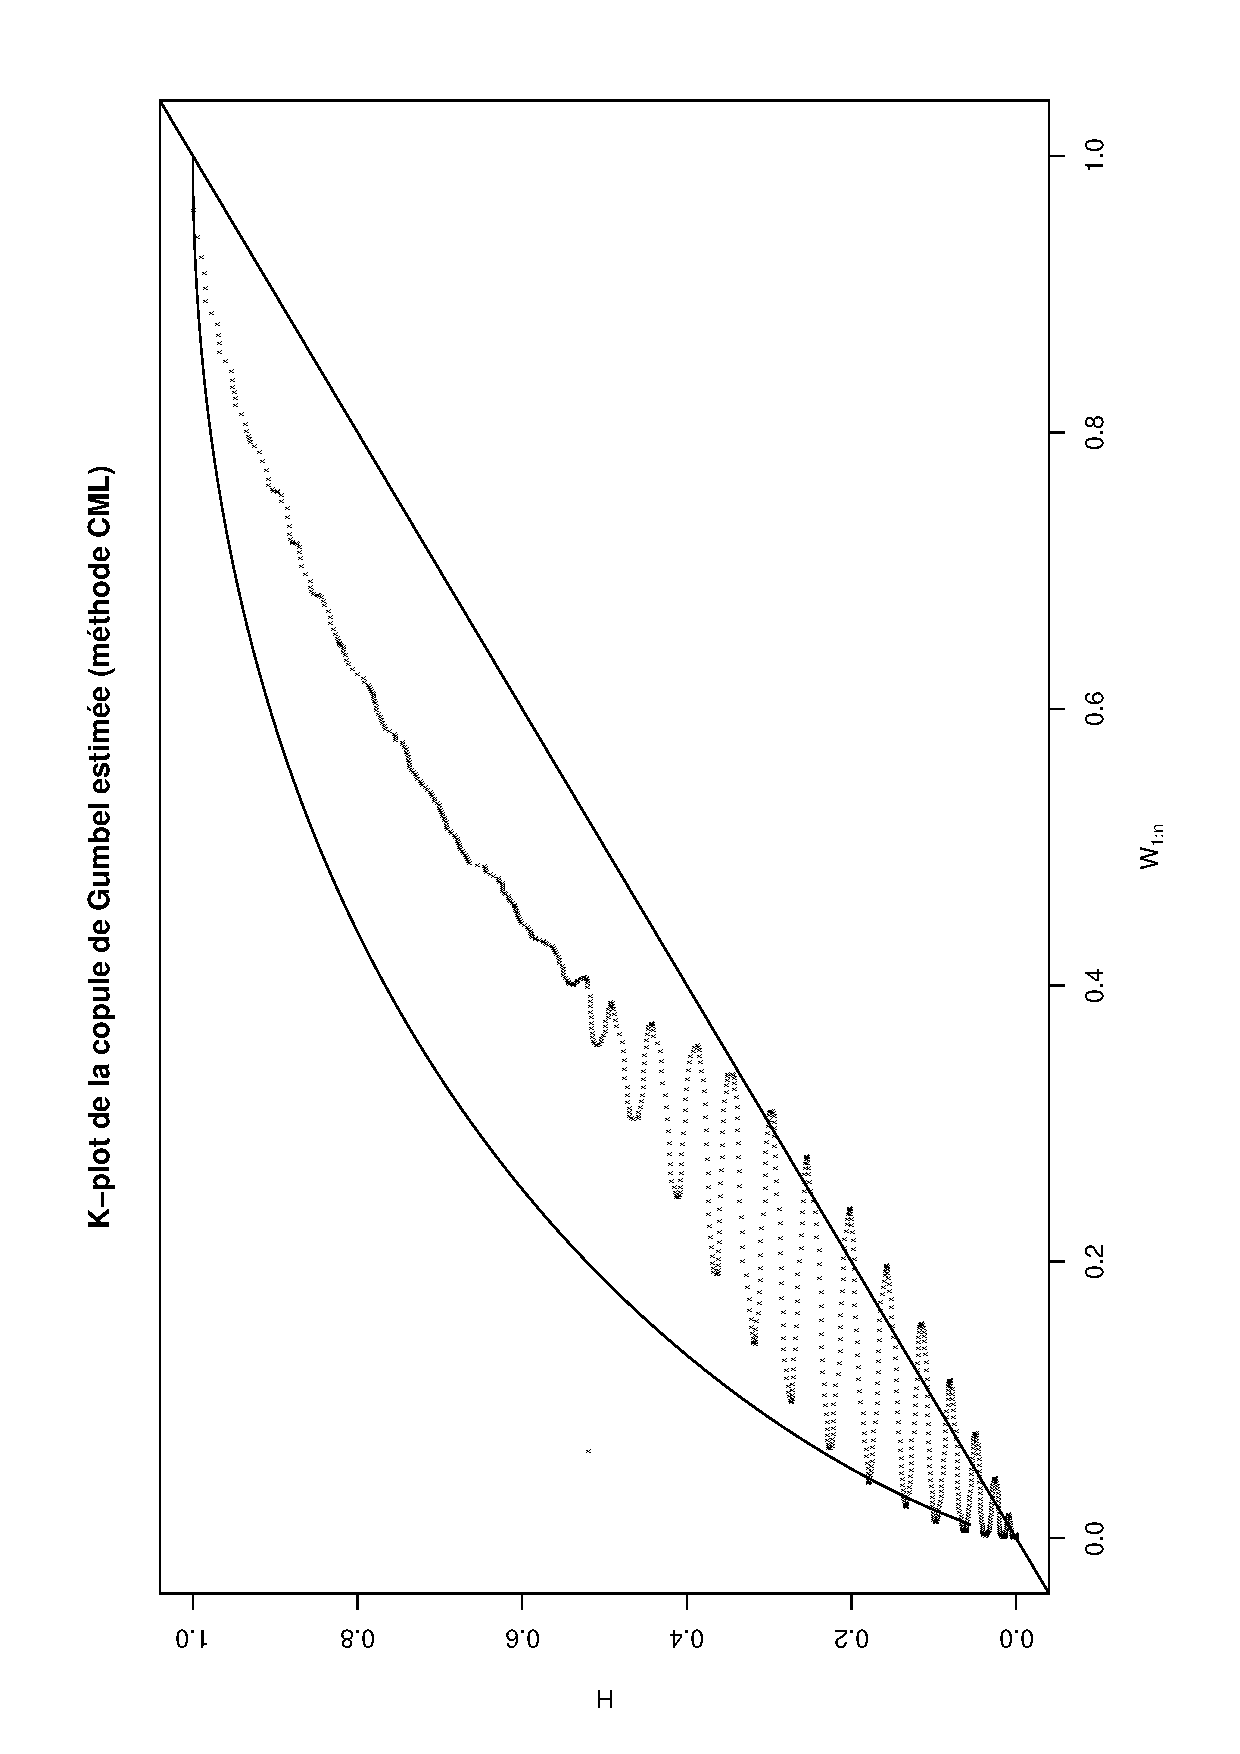
\includegraphics[width=17 cm, angle=0]{./pictures/gumbelcmlkplot.png}
      \centering\caption{\label{2}K-plot de la copule de Gumbel estimée (méthode CML)}
    \end{center}
\end{figure}

Le K-plot de la copule de Gumbel estimée et celui de la copule empirique sont très proches. Les points se répartissent dans le même endroit du graphe (entre la droite $y=x$ et la courbe de dépendance positive parfaite). De plus, on compte le même nombre d'oscillations distinctes ($12$) et les dernières espérances de statistique d'ordre sont très proches de la courbe de dépendance positive parfaite pour les deux graphes. 

En appliquant l'algorithme du bootstrap paramétrique, on obtient, toujours pour un seuil de 0,05, $D_n = 0,0324 < 0,0325 = L$. On obtient une p-value de $0,06$. Ainsi, on accepte l'hypothèse nulle et on peut conclure que notre copule empirique fait vraisemblablement partie de la famille des copules de Gumbel.

Ces résultats sur la copule de Gumbel estimée sont satisfaisants. Mais, nous pouvons voir si d'autres copules peuvent encore mieux s'approcher de la copule empirique.

\subsection{Copule de Frank}

L'estimation du paramètre de la copule de Frank par méthode CML est $\widehat{\theta}_{CML}=3,1693$. L'écart type obtenu est plus élevé que pour les deux études précédentes mais l'estimation reste largement significative. On a $sd = 0,2797$. Le maximum de vraisemblance est égal à $76,08$. Avec cette estimation, nous pouvons simuler des données issues d'une copule de Frank ayant cette valeur de paramètre. On obtient alors les graphes du Khi-plot et K-plot de la copule de Frank estimée ci-dessous:

\noindent%
\begin{figure}[H]
    \begin{center}
      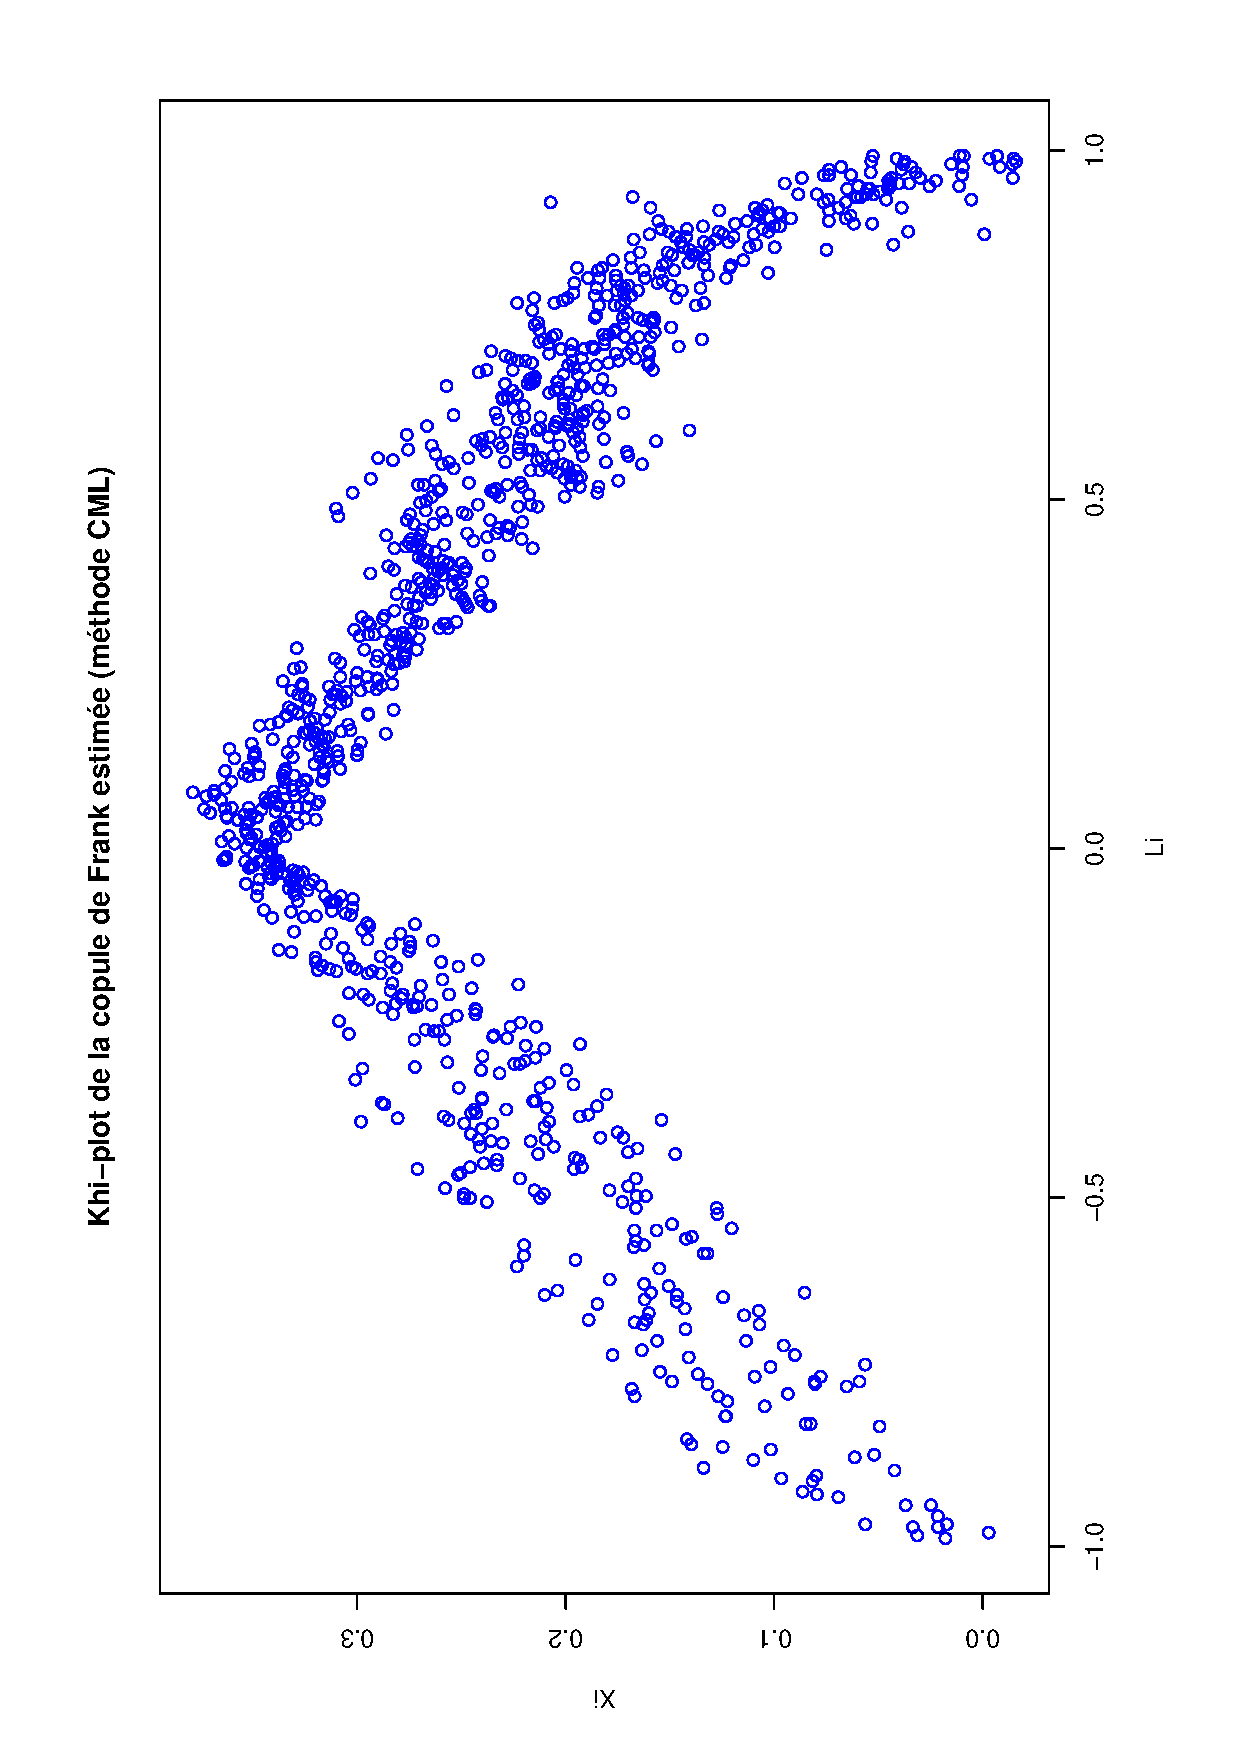
\includegraphics[width=17 cm, angle=0]{./pictures/frankcmlkhiplot.png}
      \centering\caption{\label{2}Khi-plot de la copule de Frank estimée (méthode CML)}
    \end{center}
\end{figure}

Bien que la forme du graphe ci-dessus soit proche de celui effectué pour la copule empirique, on peut remarquer plusieurs différences importantes. Tout d'abord, le Khi-plot de la copule de Frank estimée est beaucoup trop "pentu" par rapport à celui de la copule empirique. Les valeurs aux extrêmes ont une ordonnée autour de $0$ et le maximum en ordonnée dépasse les $0,3$ alors que, pour le graphe de la copule empirique, la valeur maximale en ordonnée est autour de $0,3$ et les valeurs aux extrêmes en abscisse sont autour de $0,1$.

\noindent%
\begin{figure}[H]
    \begin{center}
      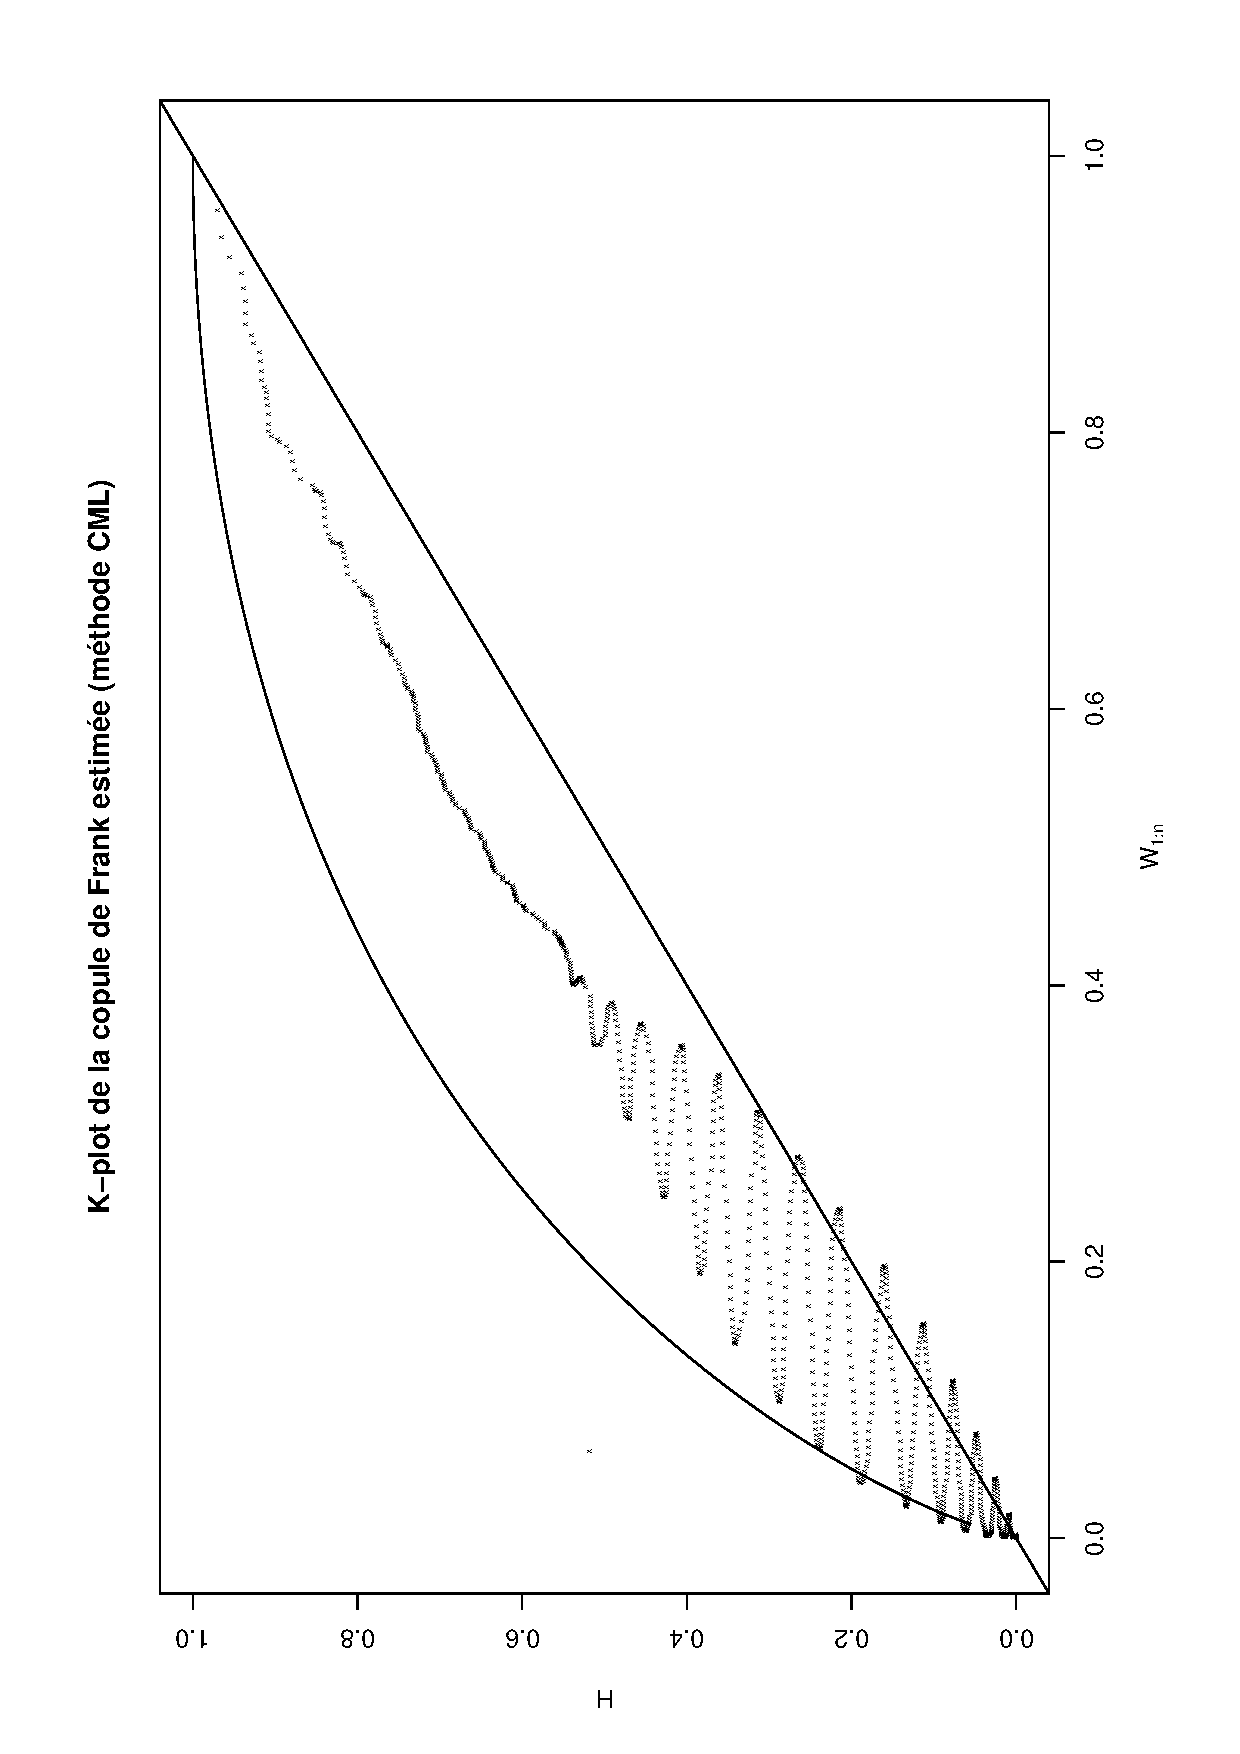
\includegraphics[width=17 cm, angle=0]{./pictures/frankcmlkplot.png}
      \centering\caption{\label{2}K-plot de la copule de Frank estimée (méthode CML)}
    \end{center}
\end{figure}

Le K-plot de la copule de Frank est assez similaire à celui de la copule de Clayton et présente donc les mêmes disparités par rapport à celui de la copule empirique. La différence la plus importante est que, pour les dernières espérances de statistique d'ordre, les points se rapprochent de la droite $y=x$ alors qu'ils sont proches de la courbe de dépendance positive parfaite pour le graphe concernant la copule empirique.

Ces graphes du Khi-plot et K-plot sont donc assez éloignés de ceux obtenus pour la copule empirique.

Cela est confirmé par l'algorithme du bootstrap paramétrique. On obtient $D_n = 0,049 > 0,025 = L$, pour un seuil de $0,05$. La p-value est nulle. Ainsi, on rejette l'hypothèse nulle et on conclut que la copule empirique ne fait pas partie de la famille des copules de Frank.

\subsection{Copule normale}

Par la méthode CML, on obtient l'estimation suivante du paramètre de la copule normale: $\widehat{\theta}_{CML}=0,5110$. L'écrat type associé vaut $sd = 0,031$, ce qui prouve la significativité de l'estimation obtenue. On obtient $93,48$ comme maximum de vraisemblance. 

Comme dans les études précédentes, on trace le Khi-plot et K-plot de la copule normale estimée et on les compare à ceux de la copule empirique.

\noindent%
\begin{figure}[H]
    \begin{center}
      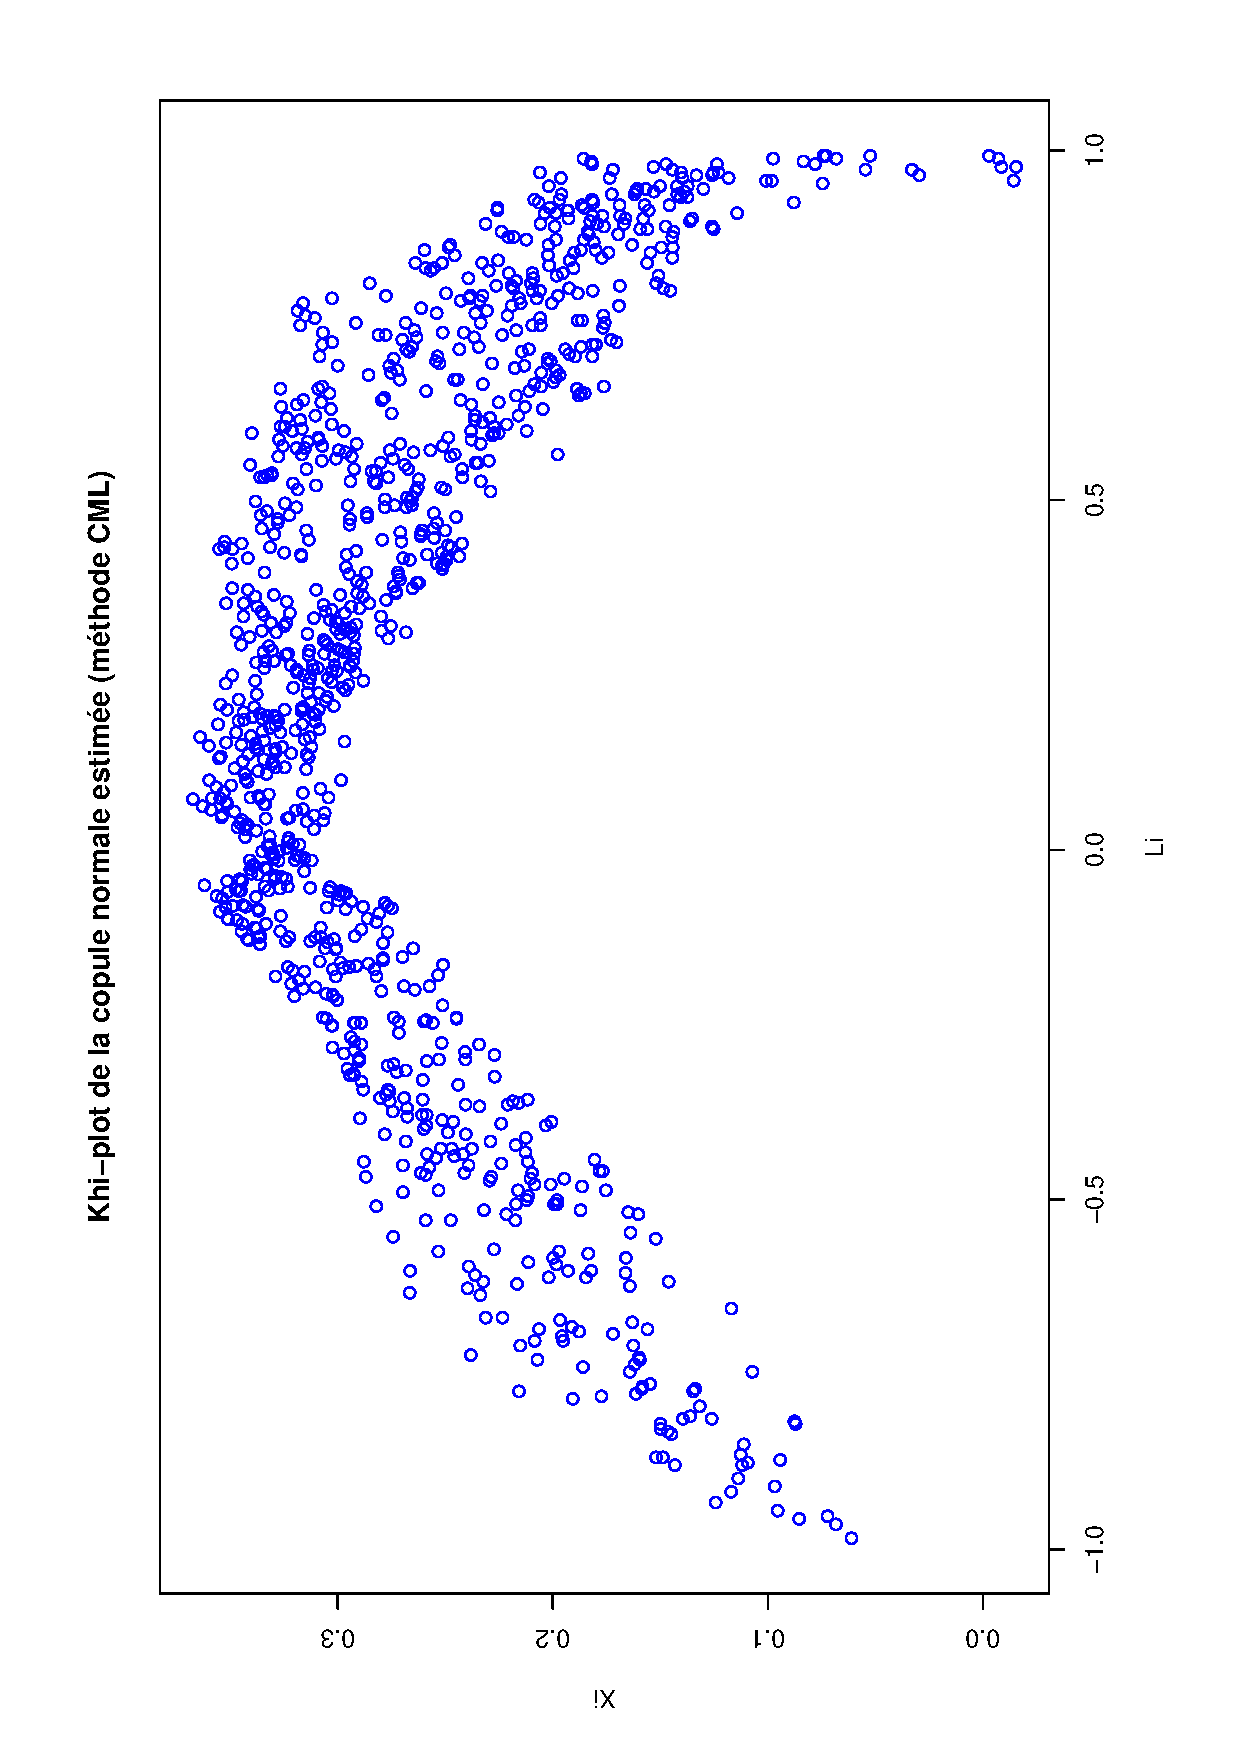
\includegraphics[width=17 cm, angle=0]{./pictures/normalcmlkhiplot.png}
      \centering\caption{\label{2}Khi-plot de la copule normale estimée (méthode CML)}
    \end{center}
\end{figure}

Le Khi-plot de la copule normale estimée est très proche de celui de la copule empirique. On retrouve, sur les deux graphes, la même forme globale du nuage de points. De plus, pour les deux, le maximum en ordonnée est autour de $0,3$ et les valeurs extrêmes des abscisses ont une ordonnée autour de $0,1$. 

\noindent%
\begin{figure}[H]
    \begin{center}
      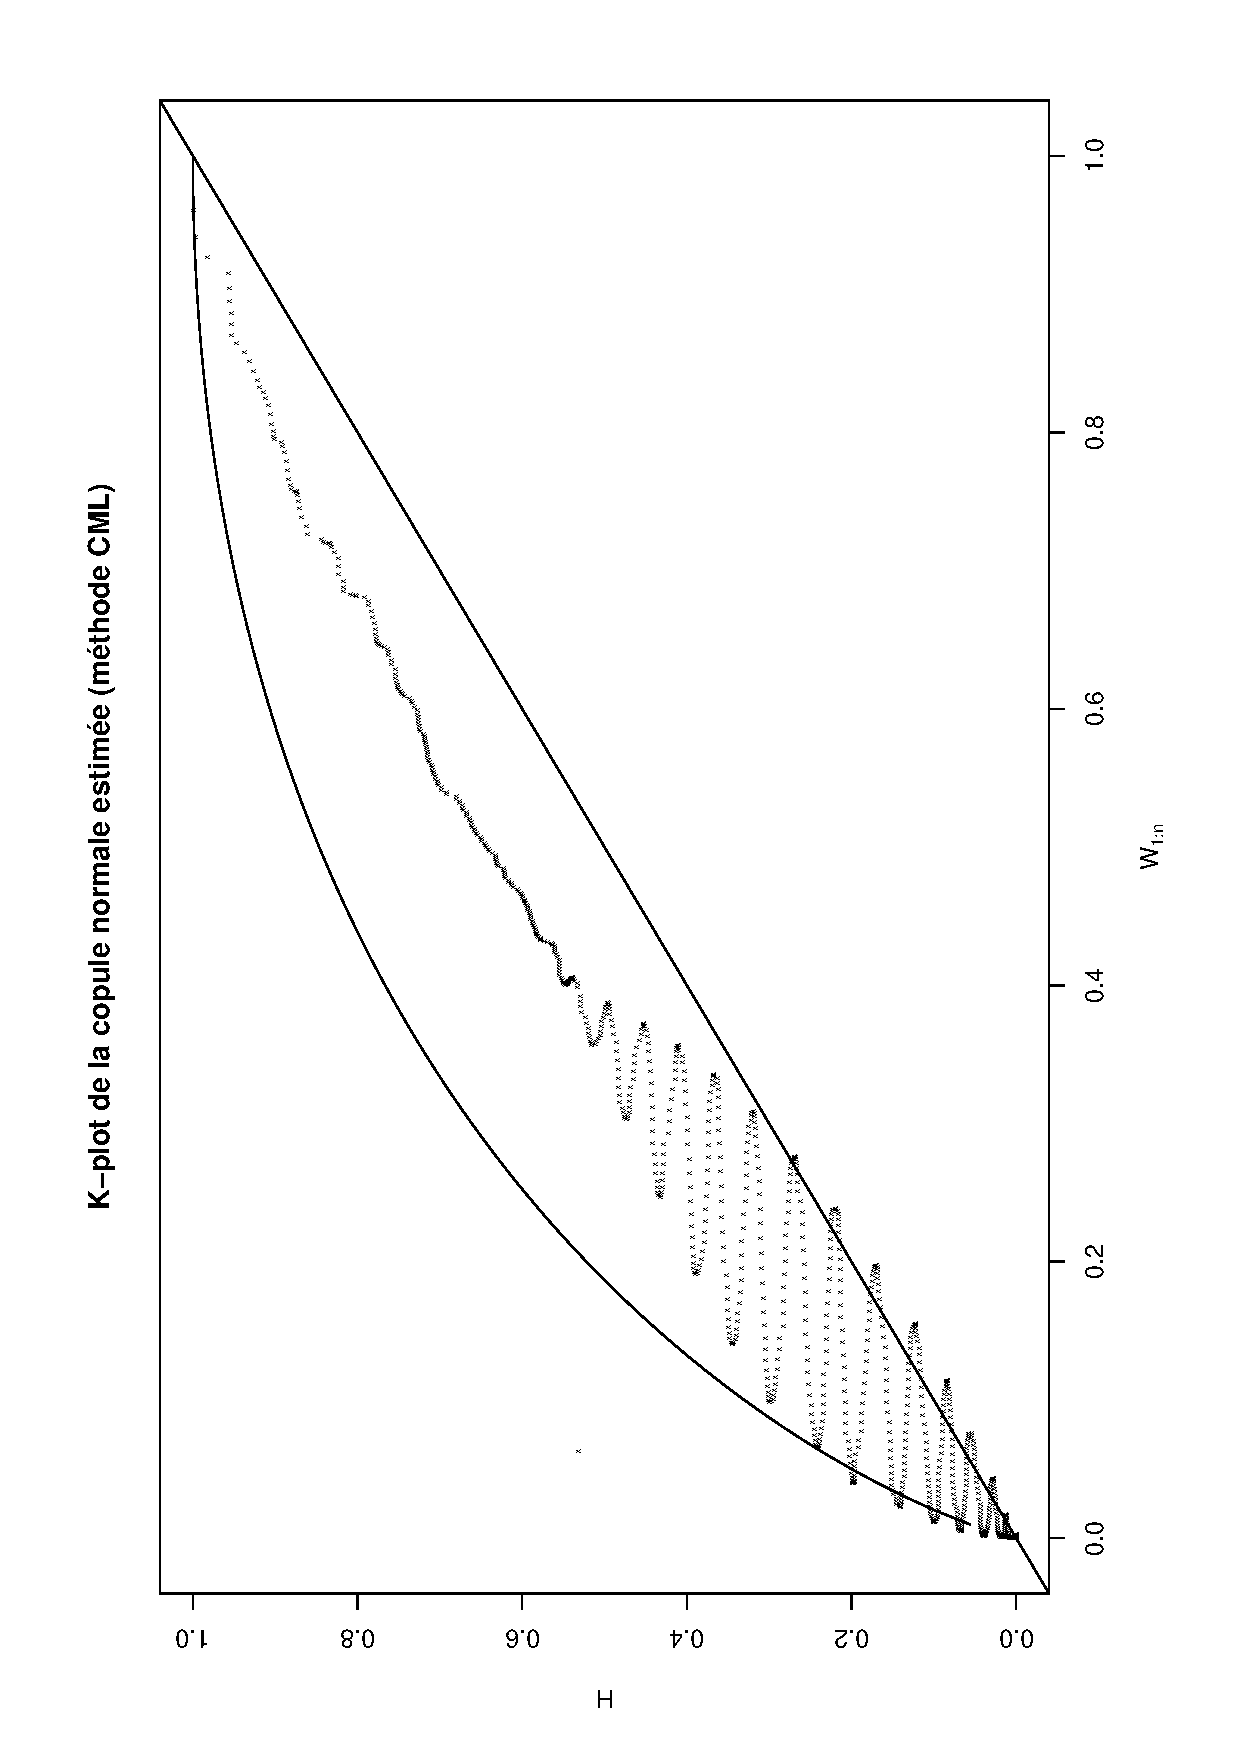
\includegraphics[width=17 cm, angle=0]{./pictures/normalcmlkplot.png}
      \centering\caption{\label{2}K-plot de la copule normale estimée (méthode CML)}
    \end{center}
\end{figure}

Concernant le K-plot de la copule normale estimée, il 

\subsection{Copule de Student}

\section{Méthode des moments : inversion du tau de Kendall}
%%%%%%%%%%%%%%%%%%%%%%%%%%%%%%%%%%%%%%%%%%%%%%%%%%%%%%%%%%%%%%%%%%%%%%%

Dans cette partie, nous utiliserons la méthode des moments pour estimer le paramètre des copules retenues afin de modéliser la dépendance entre les données sur Saint-Martin et celles sur Echirolles.

\subsection{Copule de Clayton}

\subsection{Copule de Gumbel}

\subsection{Copule de Frank}

\subsection{Copule normale}

\subsection{Copule de Student}

\section{Test graphique d'adéquation à la copule : le Kendall plot}
%%%%%%%%%%%%%%%%%%%%%%%%%%%%%%%%%%%%%%%%%%%%%%%%%%%%%%%%%%%%%%%%%%%%%%%

\subsection{Dépendogramme empirique et dépendogramme théorique}

\subsection{K-plot}

\section{Test statistique d'adéquation à la copule : le Kendall plot}
%%%%%%%%%%%%%%%%%%%%%%%%%%%%%%%%%%%%%%%%%%%%%%%%%%%%%%%%%%%%%%%%%%%%%%%

\subsection{Test de Kolmogorov-Smirnov}

\subsection{La statistique de Cramér-von Mises}

\subsection{Estimation du seuil critique par bootstrap paramétrique}





TODO   TODO   TODO   TODO



%% \noindent%
%% \begin{figure}[H]
%%     \begin{center}
%%       \includegraphics[width=17 cm, angle=0]{./pictures/logchrono1.png}
%%       \centering\caption{\label{2}Logarithme du total des importations de gaz naturel}
%%     \end{center}
%% \end{figure}
